\section*{Výsledky měření}
Kalibraci jsme provedli pomocí $^{241}$Am při vyčerpané komoře.
Pík na \SI{5485.74}{\keV} měl pološířku \SI{110}{\keV}. Rozlišení spektrometru v okolí tohoto píku je tedy \SI{110.0(5)}{\keV}, tedy \SI{2}{\percent}.

Aktivitu $a$ jsme naměřili \SI{83.5(5)}{cps}. 
Kruhový terčík byl od vzorku vzdálen $r=\SI{3.0(5)}{\cm}$ a měl plochu $S=\SI{452(40)}{\mm\squared}$
Podle \eqref{aktivita} jsme určili absolutní aktivitu vzorku
\begin{equation*}
A=\SI{2000(200)}{\becquerel}
\end{equation*}

Měření při všech tlacích probíhala \SI{300}{\s} a celkový výtěžek byl vždy v rozmezí \num{24800}--\num{25400}. Pomocí \eqref{chyba} jsme vypočetli nejistotu každého středu píku a pohybuje se v rozmezí \num{0.25}--\SI{0.50}{\keV}, takže je zcela zanedbatelná pro naše účely. Nejistotu tlaku odhadujeme na \SI{10}{\hecto\pascal}.

Do grafu \ref{g:deltaT} jsme vykreslili závislost ionizačních ztrát $\Delta T(P)=T(0)-T(P)$, závislost $T(P)$ je pouze posunutá a s opačným znamínkem. Tuto závislost jsme nafitovali funkcí $ax+bx^2+cx^3$ (bez absolutního členu, aby bylo splněno $\Delta T(0)=0$)
\begin{equation*}
\Delta T(P)=\num{-3.27}\cdot P +0.0016 \cdot P^2 -\num{1.7e-6} \cdot P^3
\end{equation*}
pokud dosazujeme $P$ v jednotkách \si{\hecto\pascal} a $T$ v \si{\keV}.

Dále jsme spočítali $f(T)$ podle \eqref{f} a \eqref{dTdP}, výsledky jsou v grafu \ref{g:f}.



\begin{tabulka}[htbp]
\centering
\begin{tabular}{c|cc}
$P$ (\si{\hecto\Pa}) & $T$ (\si{\keV}) & FWHM (\si{\keV}) \\\hline
\num{0}  &\num{5485.74} & \num{110.07} \\ 
\num{100}&\num{5157.09} & \num{109.15} \\ 
\num{200}&\num{4885.78} & \num{106.8} \\ 
\num{300}&\num{4608.68} & \num{112.43} \\ 
\num{400}&\num{4339.77} & \num{107.47} \\ 
\num{500}&\num{4031.14} & \num{122.11} \\ 
\num{600}&\num{3733.13} & \num{123.86} \\ 
\num{700}&\num{3394.79} & \num{135.83} \\ 
\num{800}&\num{3038.95} & \num{145.19} \\ 
\num{900}&\num{2593.76} & \num{164.2} \\ 
\num{960}&\num{2317.31} & \num{178.31} \\ 
\hline
\end{tabular}
\caption{Naměřené píky při různých tlacích}
\label{t:vysledky}
\end{tabulka}



\begin{graph}[htbp] 
\centering
\import{datos/}{DTP.tex}
\caption{Ionizační ztráty v závislosti na tlaku}
\label{g:deltaT}
\end{graph}

\begin{graph}[htbp] 
\centering
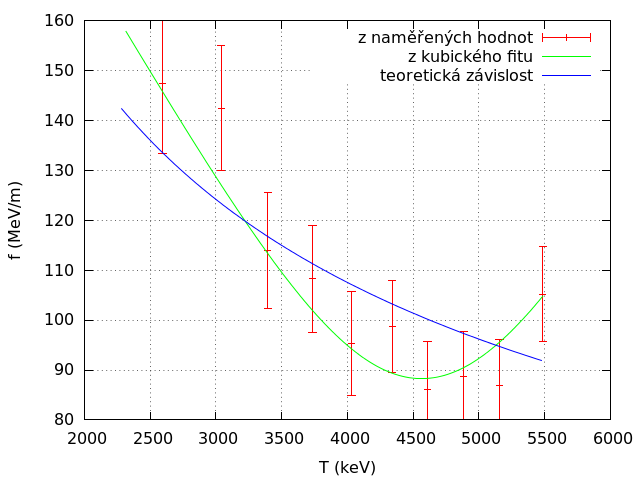
\includegraphics[width=\textwidth-2cm]{datos/f.png}
\caption{Specifické ionizační ztráty}
\label{g:f}
\end{graph}

Měřili jsme spektrum vzorku \Pudev~s příměsí \Puosm, výsledky jsou v tabulce \ref{t:vysledkyPu}. Podle \eqref{Pu} jsme spočítali jejich poměr
\begin{equation*}
\frac{N(^{238}\text{Pu})}{N(^{239}\text{Pu})}= (\num{3.8(3)})\cdot\num{e-5} \,.
\end{equation*}
Z toho máme relativní zastoupení 
\begin{equation*}
\eta(^{238}\text{Pu}) = \SI{0.0038(3)}{\percent}
 \,, \qquad \qquad \eta(^{239}\text{Pu} = \SI{99.996(1)}{\percent}
\end{equation*}







\begin{tabulka}[htbp]
\centering
\begin{tabular}{c|ccc|cc}
izotop & $T$ (\si{\keV}) & FWHM (\si{\keV}) & výtěžek (cps) & $T_{1/2}$ (\si{yr}) & $T_{\text{tab}}$ (\si{\keV}) \\\hline
\Pudev  &\num{5136.0(4)} & \num{110.07} & \num{16910(130)} & \num{24130} & \num{5142.90} \\ 
\Puosm  &\num{5475(3)} & \num{109.15} &   \num{178(14)}  & \num{87.71}  & \num{5499.21} \\ 

\hline
\end{tabular}
\caption{Naměřené píky plutonia}
\label{t:vysledkyPu}
\end{tabulka}



